% Options for packages loaded elsewhere
\PassOptionsToPackage{unicode}{hyperref}
\PassOptionsToPackage{hyphens}{url}
%
\documentclass[
]{book}
\usepackage{amsmath,amssymb}
\usepackage{iftex}
\ifPDFTeX
  \usepackage[T1]{fontenc}
  \usepackage[utf8]{inputenc}
  \usepackage{textcomp} % provide euro and other symbols
\else % if luatex or xetex
  \usepackage{unicode-math} % this also loads fontspec
  \defaultfontfeatures{Scale=MatchLowercase}
  \defaultfontfeatures[\rmfamily]{Ligatures=TeX,Scale=1}
\fi
\usepackage{lmodern}
\ifPDFTeX\else
  % xetex/luatex font selection
\fi
% Use upquote if available, for straight quotes in verbatim environments
\IfFileExists{upquote.sty}{\usepackage{upquote}}{}
\IfFileExists{microtype.sty}{% use microtype if available
  \usepackage[]{microtype}
  \UseMicrotypeSet[protrusion]{basicmath} % disable protrusion for tt fonts
}{}
\makeatletter
\@ifundefined{KOMAClassName}{% if non-KOMA class
  \IfFileExists{parskip.sty}{%
    \usepackage{parskip}
  }{% else
    \setlength{\parindent}{0pt}
    \setlength{\parskip}{6pt plus 2pt minus 1pt}}
}{% if KOMA class
  \KOMAoptions{parskip=half}}
\makeatother
\usepackage{xcolor}
\usepackage{color}
\usepackage{fancyvrb}
\newcommand{\VerbBar}{|}
\newcommand{\VERB}{\Verb[commandchars=\\\{\}]}
\DefineVerbatimEnvironment{Highlighting}{Verbatim}{commandchars=\\\{\}}
% Add ',fontsize=\small' for more characters per line
\usepackage{framed}
\definecolor{shadecolor}{RGB}{248,248,248}
\newenvironment{Shaded}{\begin{snugshade}}{\end{snugshade}}
\newcommand{\AlertTok}[1]{\textcolor[rgb]{0.94,0.16,0.16}{#1}}
\newcommand{\AnnotationTok}[1]{\textcolor[rgb]{0.56,0.35,0.01}{\textbf{\textit{#1}}}}
\newcommand{\AttributeTok}[1]{\textcolor[rgb]{0.13,0.29,0.53}{#1}}
\newcommand{\BaseNTok}[1]{\textcolor[rgb]{0.00,0.00,0.81}{#1}}
\newcommand{\BuiltInTok}[1]{#1}
\newcommand{\CharTok}[1]{\textcolor[rgb]{0.31,0.60,0.02}{#1}}
\newcommand{\CommentTok}[1]{\textcolor[rgb]{0.56,0.35,0.01}{\textit{#1}}}
\newcommand{\CommentVarTok}[1]{\textcolor[rgb]{0.56,0.35,0.01}{\textbf{\textit{#1}}}}
\newcommand{\ConstantTok}[1]{\textcolor[rgb]{0.56,0.35,0.01}{#1}}
\newcommand{\ControlFlowTok}[1]{\textcolor[rgb]{0.13,0.29,0.53}{\textbf{#1}}}
\newcommand{\DataTypeTok}[1]{\textcolor[rgb]{0.13,0.29,0.53}{#1}}
\newcommand{\DecValTok}[1]{\textcolor[rgb]{0.00,0.00,0.81}{#1}}
\newcommand{\DocumentationTok}[1]{\textcolor[rgb]{0.56,0.35,0.01}{\textbf{\textit{#1}}}}
\newcommand{\ErrorTok}[1]{\textcolor[rgb]{0.64,0.00,0.00}{\textbf{#1}}}
\newcommand{\ExtensionTok}[1]{#1}
\newcommand{\FloatTok}[1]{\textcolor[rgb]{0.00,0.00,0.81}{#1}}
\newcommand{\FunctionTok}[1]{\textcolor[rgb]{0.13,0.29,0.53}{\textbf{#1}}}
\newcommand{\ImportTok}[1]{#1}
\newcommand{\InformationTok}[1]{\textcolor[rgb]{0.56,0.35,0.01}{\textbf{\textit{#1}}}}
\newcommand{\KeywordTok}[1]{\textcolor[rgb]{0.13,0.29,0.53}{\textbf{#1}}}
\newcommand{\NormalTok}[1]{#1}
\newcommand{\OperatorTok}[1]{\textcolor[rgb]{0.81,0.36,0.00}{\textbf{#1}}}
\newcommand{\OtherTok}[1]{\textcolor[rgb]{0.56,0.35,0.01}{#1}}
\newcommand{\PreprocessorTok}[1]{\textcolor[rgb]{0.56,0.35,0.01}{\textit{#1}}}
\newcommand{\RegionMarkerTok}[1]{#1}
\newcommand{\SpecialCharTok}[1]{\textcolor[rgb]{0.81,0.36,0.00}{\textbf{#1}}}
\newcommand{\SpecialStringTok}[1]{\textcolor[rgb]{0.31,0.60,0.02}{#1}}
\newcommand{\StringTok}[1]{\textcolor[rgb]{0.31,0.60,0.02}{#1}}
\newcommand{\VariableTok}[1]{\textcolor[rgb]{0.00,0.00,0.00}{#1}}
\newcommand{\VerbatimStringTok}[1]{\textcolor[rgb]{0.31,0.60,0.02}{#1}}
\newcommand{\WarningTok}[1]{\textcolor[rgb]{0.56,0.35,0.01}{\textbf{\textit{#1}}}}
\usepackage{longtable,booktabs,array}
\usepackage{calc} % for calculating minipage widths
% Correct order of tables after \paragraph or \subparagraph
\usepackage{etoolbox}
\makeatletter
\patchcmd\longtable{\par}{\if@noskipsec\mbox{}\fi\par}{}{}
\makeatother
% Allow footnotes in longtable head/foot
\IfFileExists{footnotehyper.sty}{\usepackage{footnotehyper}}{\usepackage{footnote}}
\makesavenoteenv{longtable}
\usepackage{graphicx}
\makeatletter
\def\maxwidth{\ifdim\Gin@nat@width>\linewidth\linewidth\else\Gin@nat@width\fi}
\def\maxheight{\ifdim\Gin@nat@height>\textheight\textheight\else\Gin@nat@height\fi}
\makeatother
% Scale images if necessary, so that they will not overflow the page
% margins by default, and it is still possible to overwrite the defaults
% using explicit options in \includegraphics[width, height, ...]{}
\setkeys{Gin}{width=\maxwidth,height=\maxheight,keepaspectratio}
% Set default figure placement to htbp
\makeatletter
\def\fps@figure{htbp}
\makeatother
\setlength{\emergencystretch}{3em} % prevent overfull lines
\providecommand{\tightlist}{%
  \setlength{\itemsep}{0pt}\setlength{\parskip}{0pt}}
\setcounter{secnumdepth}{5}
\usepackage{booktabs}
\ifLuaTeX
  \usepackage{selnolig}  % disable illegal ligatures
\fi
\usepackage[]{natbib}
\bibliographystyle{plainnat}
\IfFileExists{bookmark.sty}{\usepackage{bookmark}}{\usepackage{hyperref}}
\IfFileExists{xurl.sty}{\usepackage{xurl}}{} % add URL line breaks if available
\urlstyle{same}
\hypersetup{
  pdftitle={Statistical Programming for the Social Sciences Using R},
  pdfauthor={Wesley Stubenbord},
  hidelinks,
  pdfcreator={LaTeX via pandoc}}

\title{Statistical Programming for the Social Sciences Using R}
\author{Wesley Stubenbord}
\date{2024-01-28}

\begin{document}
\maketitle

{
\setcounter{tocdepth}{1}
\tableofcontents
}
\hypertarget{about}{%
\chapter{About}\label{about}}

This is a \emph{sample} book written in \textbf{Markdown}. You can use anything that Pandoc's Markdown supports; for example, a math equation \(a^2 + b^2 = c^2\).

\hypertarget{usage}{%
\section{Usage}\label{usage}}

Each \textbf{bookdown} chapter is an .Rmd file, and each .Rmd file can contain one (and only one) chapter. A chapter \emph{must} start with a first-level heading: \texttt{\#\ A\ good\ chapter}, and can contain one (and only one) first-level heading.

Use second-level and higher headings within chapters like: \texttt{\#\#\ A\ short\ section} or \texttt{\#\#\#\ An\ even\ shorter\ section}.

The \texttt{index.Rmd} file is required, and is also your first book chapter. It will be the homepage when you render the book.

\hypertarget{render-book}{%
\section{Render book}\label{render-book}}

You can render the HTML version of this example book without changing anything:

\begin{enumerate}
\def\labelenumi{\arabic{enumi}.}
\item
  Find the \textbf{Build} pane in the RStudio IDE, and
\item
  Click on \textbf{Build Book}, then select your output format, or select ``All formats'' if you'd like to use multiple formats from the same book source files.
\end{enumerate}

Or build the book from the R console:

\begin{Shaded}
\begin{Highlighting}[]
\NormalTok{bookdown}\SpecialCharTok{::}\FunctionTok{render\_book}\NormalTok{()}
\end{Highlighting}
\end{Shaded}

To render this example to PDF as a \texttt{bookdown::pdf\_book}, you'll need to install XeLaTeX. You are recommended to install TinyTeX (which includes XeLaTeX): \url{https://yihui.org/tinytex/}.

\hypertarget{preview-book}{%
\section{Preview book}\label{preview-book}}

As you work, you may start a local server to live preview this HTML book. This preview will update as you edit the book when you save individual .Rmd files. You can start the server in a work session by using the RStudio add-in ``Preview book'', or from the R console:

\begin{Shaded}
\begin{Highlighting}[]
\NormalTok{bookdown}\SpecialCharTok{::}\FunctionTok{serve\_book}\NormalTok{()}
\end{Highlighting}
\end{Shaded}

\hypertarget{an-introduction-to-r}{%
\chapter{An Introduction to R}\label{an-introduction-to-r}}

To get started, you will need to install two things:

\begin{enumerate}
\def\labelenumi{\arabic{enumi}.}
\item
  R, a programming language
\item
  RStudio, a software program that helps you program in R.

  \begin{itemize}
  \tightlist
  \item
    This type of software program is called an IDE, an Integrated Development Environment.
  \end{itemize}
\end{enumerate}

You don't necessarily need RStudio to program in R, but it does make life a lot easier and it is what we will be using throughout the course.

\hypertarget{installing-r}{%
\section{Installing R}\label{installing-r}}

To install R, go to \url{https://cran.irsn.fr/index.html}, select the appropriate operating system and follow the instructions.

For example, if you have a Mac, you will click on ``Download R for macOS,'' followed, in most cases, by clicking on the ``R-4.3.2-arm64.pkg'' link beneath the ``Latest release:'' header.

On the other hand, if you have a PC running Windows, you will click on ``Download R for Windows'' followed by ``install R for the first time,'' followed by ``Download R-4.3.2 for Windows.''

In either case, your browser should start downloading an executable file which you will then need to run to install R.

\emph{CAUTION}: A couple things you may need to watch out for:

\begin{enumerate}
\def\labelenumi{\arabic{enumi}.}
\item
  If you are using an older laptop, you may need to download a different version of R or RStudio. When in doubt, read the installation pages and refer to your operating system version.
\item
  If you have very little hard drive space on your computer, you may need to clear some space before you go to install RStudio. The latest RStudio version requires 215 MB and you'll need some additional space for other software and data that you will need later on in the course (around 2 GB should be enough I imagine).
\end{enumerate}

\hypertarget{installing-rstudio}{%
\section{Installing RStudio}\label{installing-rstudio}}

Once you've installed R, go to \url{https://posit.co/download/rstudio-desktop/}. Posit (a company formerly known as RStudio) offers RStudio Desktop free of charge. They also have a cloud-based version of the software (Posit Cloud) which has a free-tier and paid-tiers. If you have trouble using RStudio Desktop in this course, you may consider using a Posit Cloud account as discussed in the course syllabus.

Step 1 is already complete - you've already installed R. On the landing page linked above, you'll find different versions of RStudio according to your computer's operating system. Select the operating system that applies to your case, download the install, and then, once it has downloaded, run the installer from your computer and follow the on-screen steps. You'll be running RStudio in no time.

If all goes well, your RStudio screen should look something like this once it is correctly installed and running:

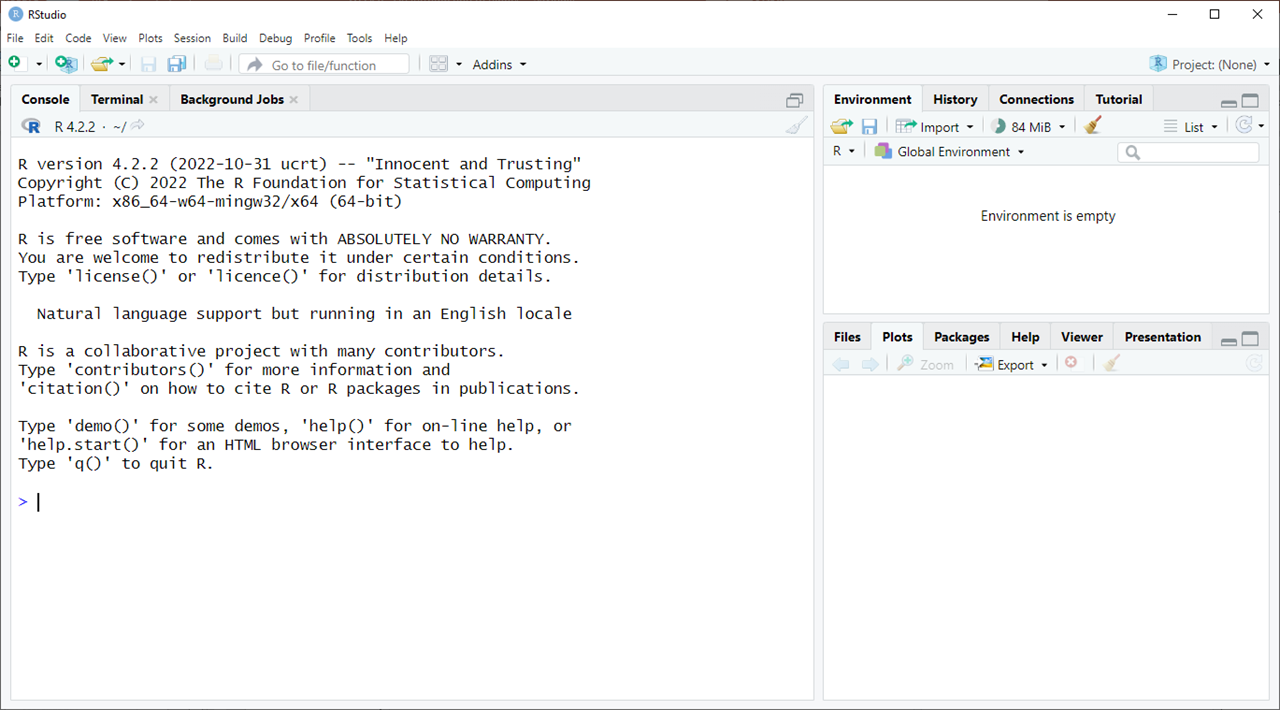
\includegraphics{docs/_main_files/figure-html/RStudio clean install.png}

Now the fun begins.

  \bibliography{book.bib,packages.bib}

\end{document}
